\documentclass[letterpaper,10pt,titlepage, onecolumn, compsoc]{IEEEtran}

\usepackage{graphicx}                                        
\usepackage{amssymb}                                         
\usepackage{amsmath}                                         
\usepackage{amsthm}                                          
\usepackage{longtable}

\usepackage{alltt}                                           
\usepackage{float}
\usepackage{color}
\usepackage{url}

\usepackage{balance}
\usepackage[TABBOTCAP, tight]{subfigure}
\usepackage{enumitem}
\usepackage{pstricks, pst-node}

\usepackage{geometry}
\geometry{textheight=8.5in, textwidth=6in}

\newcommand{\cred}[1]{{\color{red}#1}}
\newcommand{\cblue}[1]{{\color{blue}#1}}

\usepackage{hyperref}
\usepackage{geometry}

\title{Concurrency 2 \\The Look I/O Scheduler \\ \vspace{2mm}\small CS444 (Spring 2017)}
\author{Authored by \\ Nathan Shepherd, Stephen Krueger, Joshua Matteson }
\begin{document}
% Title page
\maketitle
\newpage


\section{Plans}




\section{Questions}

\subsection{What do you think the main point of this assignment is?}
The main purpose of this assignment was to engender a deeper understanding of the linux kernel modules. The code is complex and it takes a lot of hands on time to begin to understand. Implementing the IO schedulers got us acquainted with the code and how the kernel handles process scheduling.      

\subsection{How did you personally approach the problem?}

We decided to tackle the elevator work first as that seemed to be the most complicated part of the assignment. 
We were wrong. It actually took us a lot longer to get the code running on the kernel and get the output that we required. 


\subsection{How did you ensure your solution was correct?}
To ensure that our solution was correct we made sure that the code we wrote could compile and then set the kernel to use our code as the default option. We got our output and trimmed it down to just html so we could analyze our data. 

Figure \ref{fig:output1} shows our html output.


\begin{figure}[b]
	\centering
      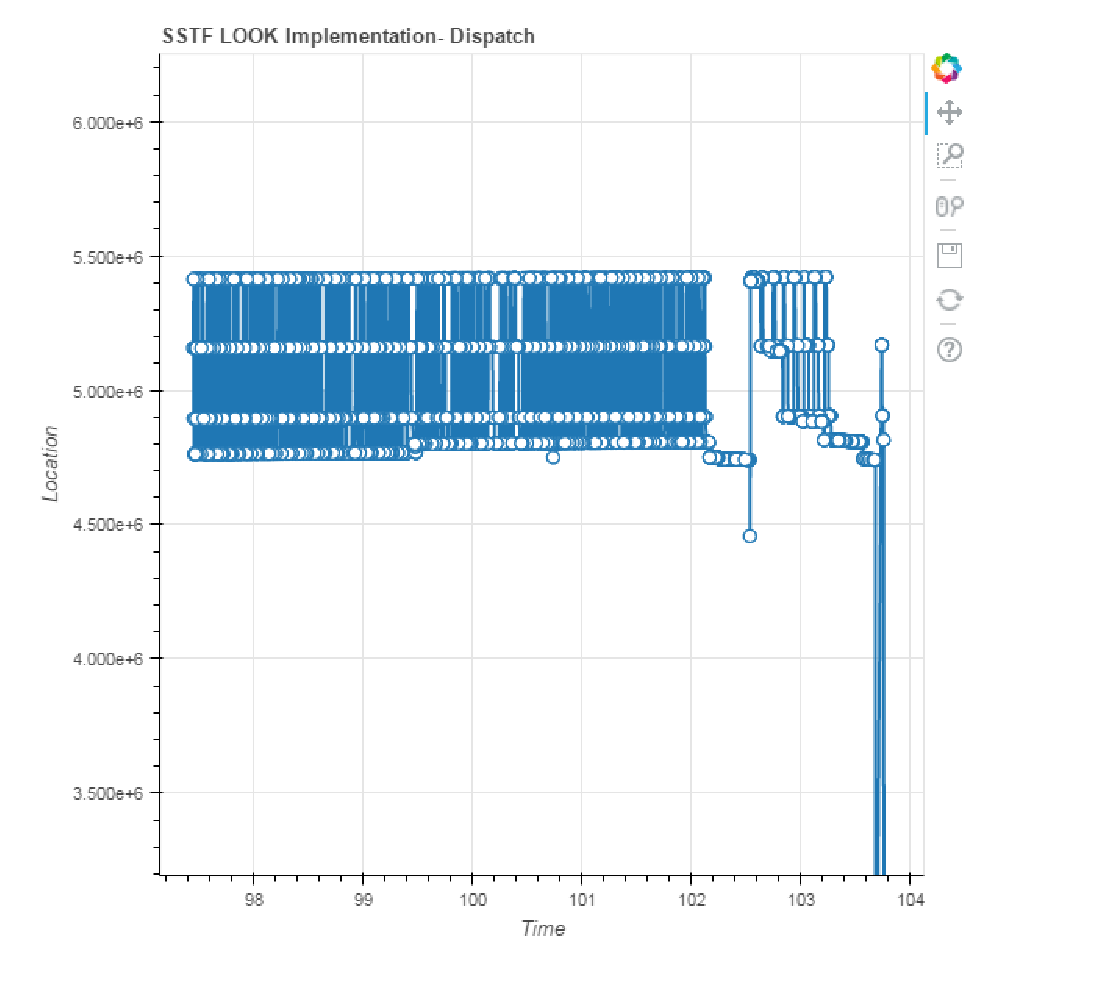
\includegraphics[]{afe.eps}
    \caption{SSTF LOOK Implementation Dispatch}
    \label{fig:output1}
\end{figure}
    

\subsection{What did you learn?}
We learned a lot about the how linux kernels handle processes and I/O operations...

\section{Version Control Log}
\begin{tabular}{lp{12cm}}
  \label{tabular:legend:git-log}
  \textbf{acronym} & \textbf{meaning} \\
  V & \texttt{version} \\
  tag & \texttt{git tag} \\
  MF & Number of \texttt{modified files}. \\
  AL & Number of \texttt{added lines}. \\
  DL & Number of \texttt{deleted lines}. \\
\end{tabular}

\bigskip

\begin{longtable}{|rlllrrr|}
\hline \multicolumn{1}{|c}{\textbf{V}} & \multicolumn{1}{c}{\textbf{tag}}
& \multicolumn{1}{c}{\textbf{date}}
& \multicolumn{1}{c}{\textbf{commit message}} & \multicolumn{1}{c}{\textbf{MF}}
& \multicolumn{1}{c}{\textbf{AL}} & \multicolumn{1}{c|}{\textbf{DL}} \\ \hline
\endhead

\hline \multicolumn{7}{|r|}{} \\ \hline
\endfoot

\hline% \hline
\endlastfoot

\hline 1 &  & 2017-04-20 & Logs and kernel hw1 & 45934 & 18287987 & 0 \\
\hline 2 &  & 2017-04-27 & Added a gitignore & 1 & 1 & 0 \\
\hline 3 &  & 2017-04-27 & Added qemu\_command script & 1 & 3 & 0 \\
\hline 4 &  & 2017-04-27 & Added sstf file & 2 & 125 & 0 \\
\hline 5 &  & 2017-05-03 & assign1 folder, starting on assign2 & 5 & 6054 & 2 \\
\hline 6 &  & 2017-05-03 & Current linux working & 1 & 0 & 1 \\
\hline 7 &  & 2017-05-03 & Bash runner now uses correct scheduler & 4 & 39 & 39 \\
\hline 8 &  & 2017-05-07 & Implemented C-LOOK & 1 & 84 & 20 \\
\end{longtable}

 
\section{Work Log}
\begin{itemize}
\item Thursday 4th - Got started on the Concurrency part of the assignment in the recitation.
\item Friday 5th - Started to work on the kernel assignment, finished the concurrency problem that night. 
\item Sunday 7th - Made a lot of progress on the kernel part of the assignment, still have to get files running on the kernel.  
\item Monday 8th - Finished kernel problem and finished the writeup.
\end{itemize}

\end{document}
